\chapter{Returning to Chithurst}

During my time down in Devon, Ajahn Sumedho and a substantial portion of
the sangha had moved to live near Hemel Hempstead, north of London,
where they were engaged in building a new monastery, to be called
Amaravati\cite{amaravati}. The move came about because of the
increased activity at Chithurst,
including growth within the nuns' community. After considerable
discussion a decision was made to find another place that would not only
accommodate an increasing number of resident sangha members, but could
also serve as a facility that provided resident retreats for laypeople.
Because of planning restrictions imposed by the council on the Chithurst
property, retreats for large numbers of lay guests were never going to
be possible. Hiring conference centres always felt like a bit of
compromise. It would have been alright to continue hiring conference
centres, and in some ways it might have been more convenient; however,
given the need to expand anyway, finding a much larger property seemed
sensible.

Initially, after Ajahn Sumedho left, Ajahn Tiradhammo led the community
at Chithurst; after about six months, Ajahn Anando, who had been living
in Harnham, came back to take over. For most of the year in those days
there was a small community of nuns also resident at Chithurst, in the
cottage next to Hammer Wood, but during the Rains Retreat they were all
together at Amaravati.

As the years passed, more options for spiritual development were opening
up throughout Britain, and in presumably the Western world. Teachers
within the Burmese tradition of U Ba Khin already had centres
established in Britain before we arrived. More yoga groups and
meditation groups seemed to be opening up all the time. Brockwood Park,
the Krishnamurti Centre, was just a few miles away. Still there seemed
to be a steady stream of guests passing through Chithurst, with some
asking to stay and take up monastic training. The monastery appeared to
be serving a particular need.

One of those visitors, in 1986, was Andrew Walker. Having recently
completed a degree in Comparative Religion at the university at Bristol,
he was driving back to his parents' place up in Yorkshire. He took the
opportunity to stay for three nights at the monastery, and, in
conversation with me, mentioned he was interested in taking up the
anagarika training. About two years later, in April 1988, he requested
the eight precepts of an anagarika at Amaravati. These days, as Ajahn
Puñño, he is a valued member and dear personal friend, living as part of
the sangha here at Harnham.

Also during that period while I had been in Devon, Ajahn Viradhammo had
moved to New Zealand and was busy building Bodhinyanarama Monastery in
Stokes Valley, just north of Wellington; Ajahn Tiradhammo had moved to
Harnham, in Northumberland. Towards the end of 1986, Ajahn Sumedho
invited Ajahn Anando to accompany him on an overseas teaching tour which
would include the U.S. and New Zealand. That meant I was left to lead
the sangha at Chithurst during the Winter Retreat of 1987. It surprises
me now, when I think back about that period, that I was not more
intimidated by such a turn of events. We were still in a pioneer phase
of development and there was a lot that kept changing. I can't say I
felt particularly confident, but neither was I terribly daunted. In some
ways the whole thing felt like a shared adventure. To call what we were
doing an experiment feels like it trivializes the intense effort people
were making. It was a daring exploration of the unknown inner worlds in
an increasingly secular society.

During the Rains Retreat of the previous year, Ajahn Anando and I had
spoken about the possibility of asking Ajahn Sumedho to change my name.
I had never found the name that I had been given back in 1976, `Tan
Uppanno', at all inspiring; it literally means `manifest' or `arisen'.
Compared with names such as Tan Anando, ` the great blissful one' or Tan
Sucitto, `the beautiful-hearted one', I felt just a little hard done by.
Besides, it also sounded weird. I mentioned to Ajahn Anando that one of
the other monks who took Precepts at the same time as I did, Tan Puriso,
had once asked Tan Ajahn Chah about receiving a new name. His name,
Puriso, translated as `man'. Apparently Tan Ajahn Chah had said
something like, \emph{come and see me again when you have been a monk
for ten years.} By 1987 I had been a monk for ten Rains Retreats. Also
there had recently been a notable improvement in my health, and
somewhere I had read, or heard that in certain Buddhist cultures, under
such circumstances, people might take on a new name. In the end, nothing
came out of those discussions since, as far as I recall, neither of us
was minded to approach Ajahn Sumedho about it.

Hence it came as a surprise when, part way through that Winter Retreat,
I received a card from Ajahn Anando, who was with Ajahn Sumedho
somewhere in the U.S. He explained that Ajahn Sumedho happened to
mention to him that he wanted to do something supportive for Tan
Uppanno. That gave Ajahn Anando an opening to tell him that I would be
grateful for a new name. We had already discussed a few possibilities
which Ajahn Anando was able to remember, so Ajahn Sumedho selected the
name Munindo. It was also during that Winter Retreat that the sangha of
monks at Chithurst presented me with a new robe which they had sewn.

Improved health, receiving a new name and a new robe, all gave me
strength; and I needed it. Most of the sangha members there at the time
were very new to the training, and that called for a certain quality of
attention. And leading a two-month long meditation retreat wasn't the
only thing happening; as I mentioned, there was a lot that was changing.
Along with the relocation of many community members to Amaravati, much
of the management had gone too. It was taking time to get things running
smoothly. I remember how during that retreat we received notification
that various bills, including the telephone, were not being paid (by the
administrator now located at Amaravati). Also around that time, one of
the leaders of the community of lay supporters was manoeuvring to
establish an alternative structure to the English Sangha Trust. Looking
back now, such events appear to be not such a big issue; however at the
time they did contribute to a perception of pressure. It would still be
many years before there was the option of setting up a Skype call with a
senior sangha friend, who was teaching in San Francisco and benefitting
from their counsel.

As it happened, not only did we survive, but lessons were learned, and
now I can appreciate them. It is bound to happen over and over again on
this spiritual journey, that practice will take us to the point where it
all feels too much. We have to get used to it, and stop resisting.
Saying `it shouldn't be this way' is not what Tan Ajahn Chah taught.
Rather, we need to learn how to turn perceptions of outer pressure into
inner strength and increased competence.

After Ajahn Anando returned, he, Tan Vajiro and myself settled into a
rhythm whereby the three of us took turns in visiting and giving talks
at various meditation groups that had become associated with the
monastery. Sometimes this meant going by public transport up to London;
at other times a lay friend of the monastery would drive us down to the
south-coast; Brighton or Southampton. It might have been because of one
of those teaching trips that I found myself in London on that fateful
night in October 1987, when a powerful hurricane tore through southern
England. According to a BBC article\cite{kent}, eighteen people were
killed in that storm. A couple
of days after the storm, when it came to trying to get transport back to
West Sussex, we found most of the routes were blocked. A large number of
trees had come down, resulting in a great deal of damage. Eventually I
think I managed to get a train or bus, via Heathrow, down to
Southampton, where a supporter, who was a member of the Laotian
community there, picked me up and drove me to Chithurst. From the road
approaching the monastery we could see that the massive Cedar tree,
which had once stood close to the main house, was no longer there. The
question was, which way had it fallen. Fortunately, it had fallen away
from the house. Had it gone in the opposite direction it could have
taken out at least half of the house, and possibly have caused serious
injury or even death.

On the positive side, timber from that cedar tree was milled and stored,
and eventually used to construct desktops and surfaces in the old
granary when it was converted into the abbot's residence. Perhaps even
more positively, a good number of the oak trees that had come down in
Hammer Wood were milled, dried, and, a few years later, sent up to
Harnham to form the floor of their new Dhamma Hall. I expect that all
happened because of Ajahn Anando's considerable generosity. There is no
doubt that the Harnham sangha were very grateful. Such beautiful thick
oak planks would have cost a fortune to purchase.

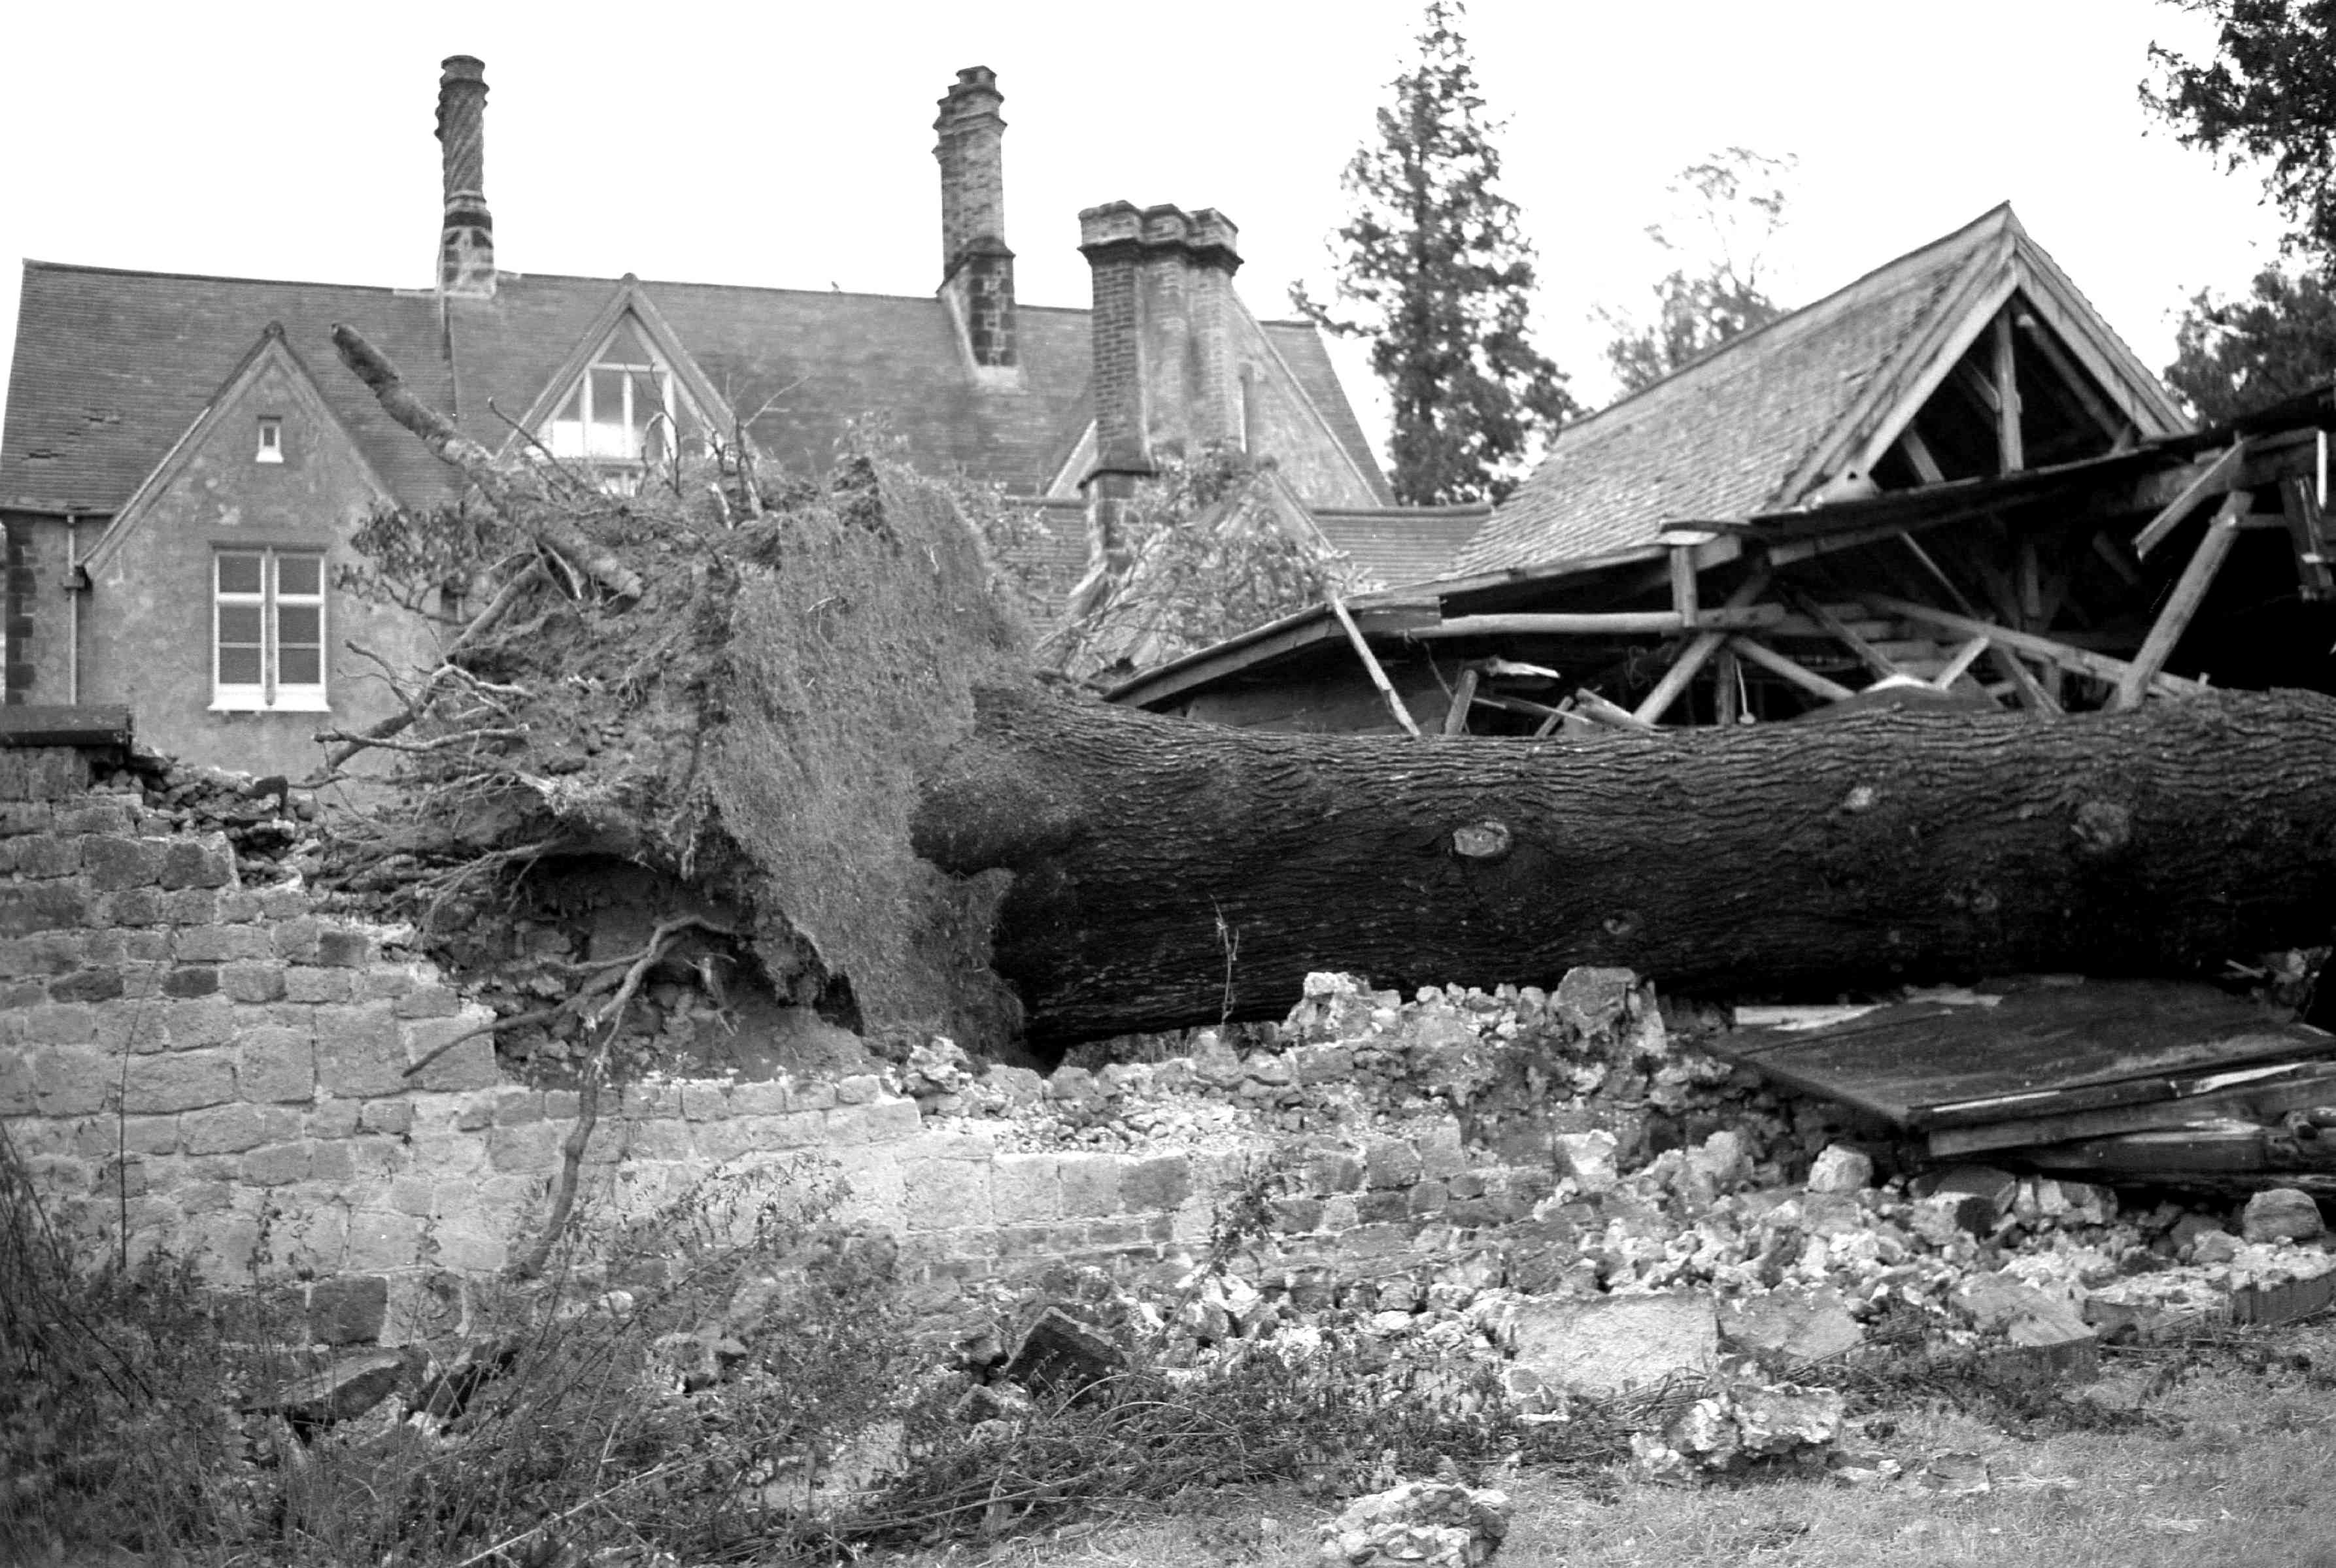
\includegraphics[width=\linewidth]{image4.jpeg}

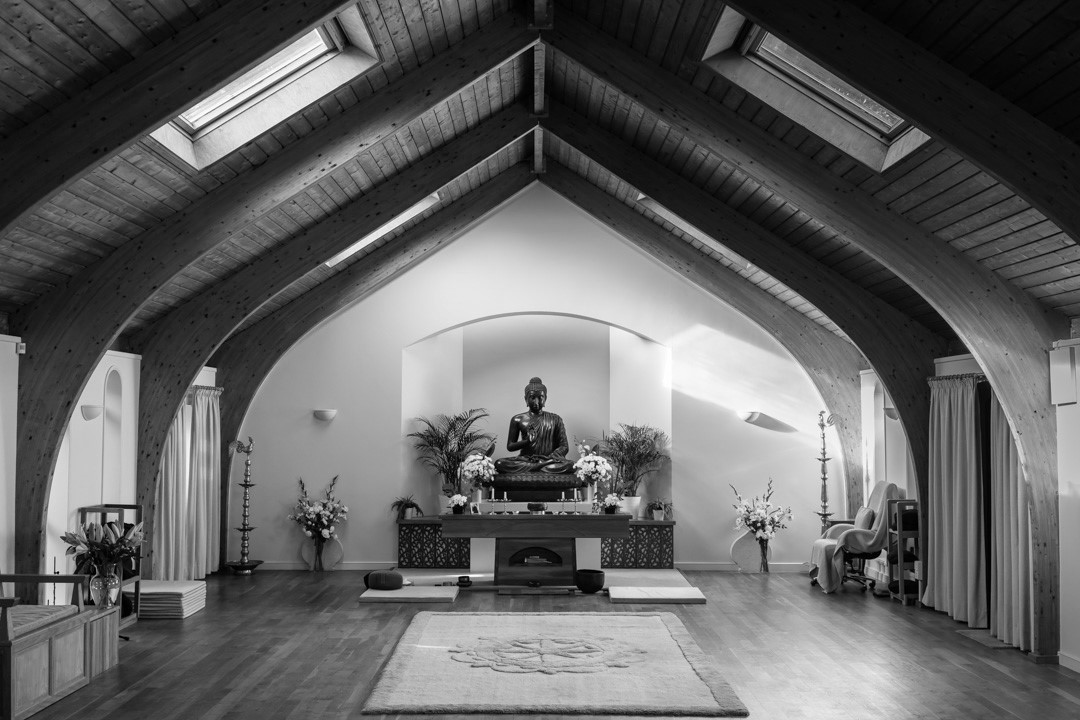
\includegraphics[width=\linewidth]{image5.jpeg}

